\documentclass[pdftex]{beamer}
\usepackage[british]{babel}
\usepackage{graphicx}
\usepackage{url}
\usepackage[normalem]{ulem}
\usepackage{tikz}

\mode<presentation>
\usetheme{Warsaw}
\useoutertheme{infolines}

\setbeamertemplate{navigation symbols}{}
% \usebeamertemplate*{logo}
% \logo{
\includegraphics[height=0.85cm]{../images/cmetlogo.png}}

\title[Measuring UK Crime Networks]{{\huge{Measuring UK Crime Networks}}}
\author[ASONAM 2014]{Giles Oatley and Tom Crick\\\url{tcrick@cardiffmet.ac.uk}}
\institute[@DrTomCrick]{Department of Computing \& Information
  Systems\\Cardiff Metropolitan University, UK\\\url{http://drtomcrick.com}}
\date{19 August 2014}

% logo  on title page only
\titlegraphic{
\includegraphics[width=4cm]{../images/cmetlogo.png}
}

\begin{document}

% titlepage
\begin{frame}
\titlepage
\end{frame}

% TOC
\section*{Talk Outline} 
\begin{frame} 
\tableofcontents 
\end{frame} 

\section{Introduction and Motivation}

\begin{frame}
\frametitle{Abstract}
{\small{{\emph{
This paper describes the output of a study to tackle the problem of
gang-related crime in the UK; we present the intelligence and
routinely gathered data available to a UK regional police force, and
describe an initial social network analysis of gangs in the Greater
Manchester area of the UK between 2000-2006.\newline

By applying social network analysis techniques, we attempt to detect
the birth of two new gangs based on local features (modularity,
cliques) and global features (clustering coefficient). Thus for the
future, identifying the changes in these can help us identify the
possible birth of new gangs (sub-networks) in the social
system.\newline

Furthermore, we study the dynamics of these networks globally and
locally, and have identified the global characteristics that tell us
that they are not random graphs -- they are small world graphs --
implying that the formation of gangs is not a random event. However,
we are not yet able to conclude anything significant about scale-free
characteristics due to insufficient sample size.}}}}
\end{frame}

\section{Gang Formation}

\begin{frame}
\frametitle{Gang Formation}
\begin{center}
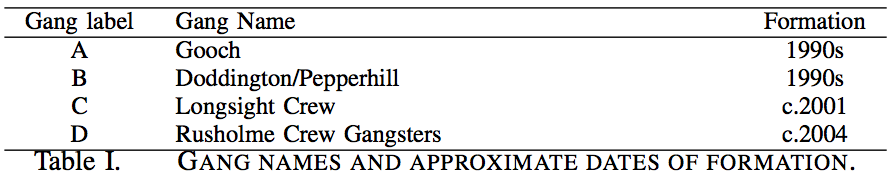
\includegraphics[width=0.8\textwidth]{../images/gangs.png}\newline\newline
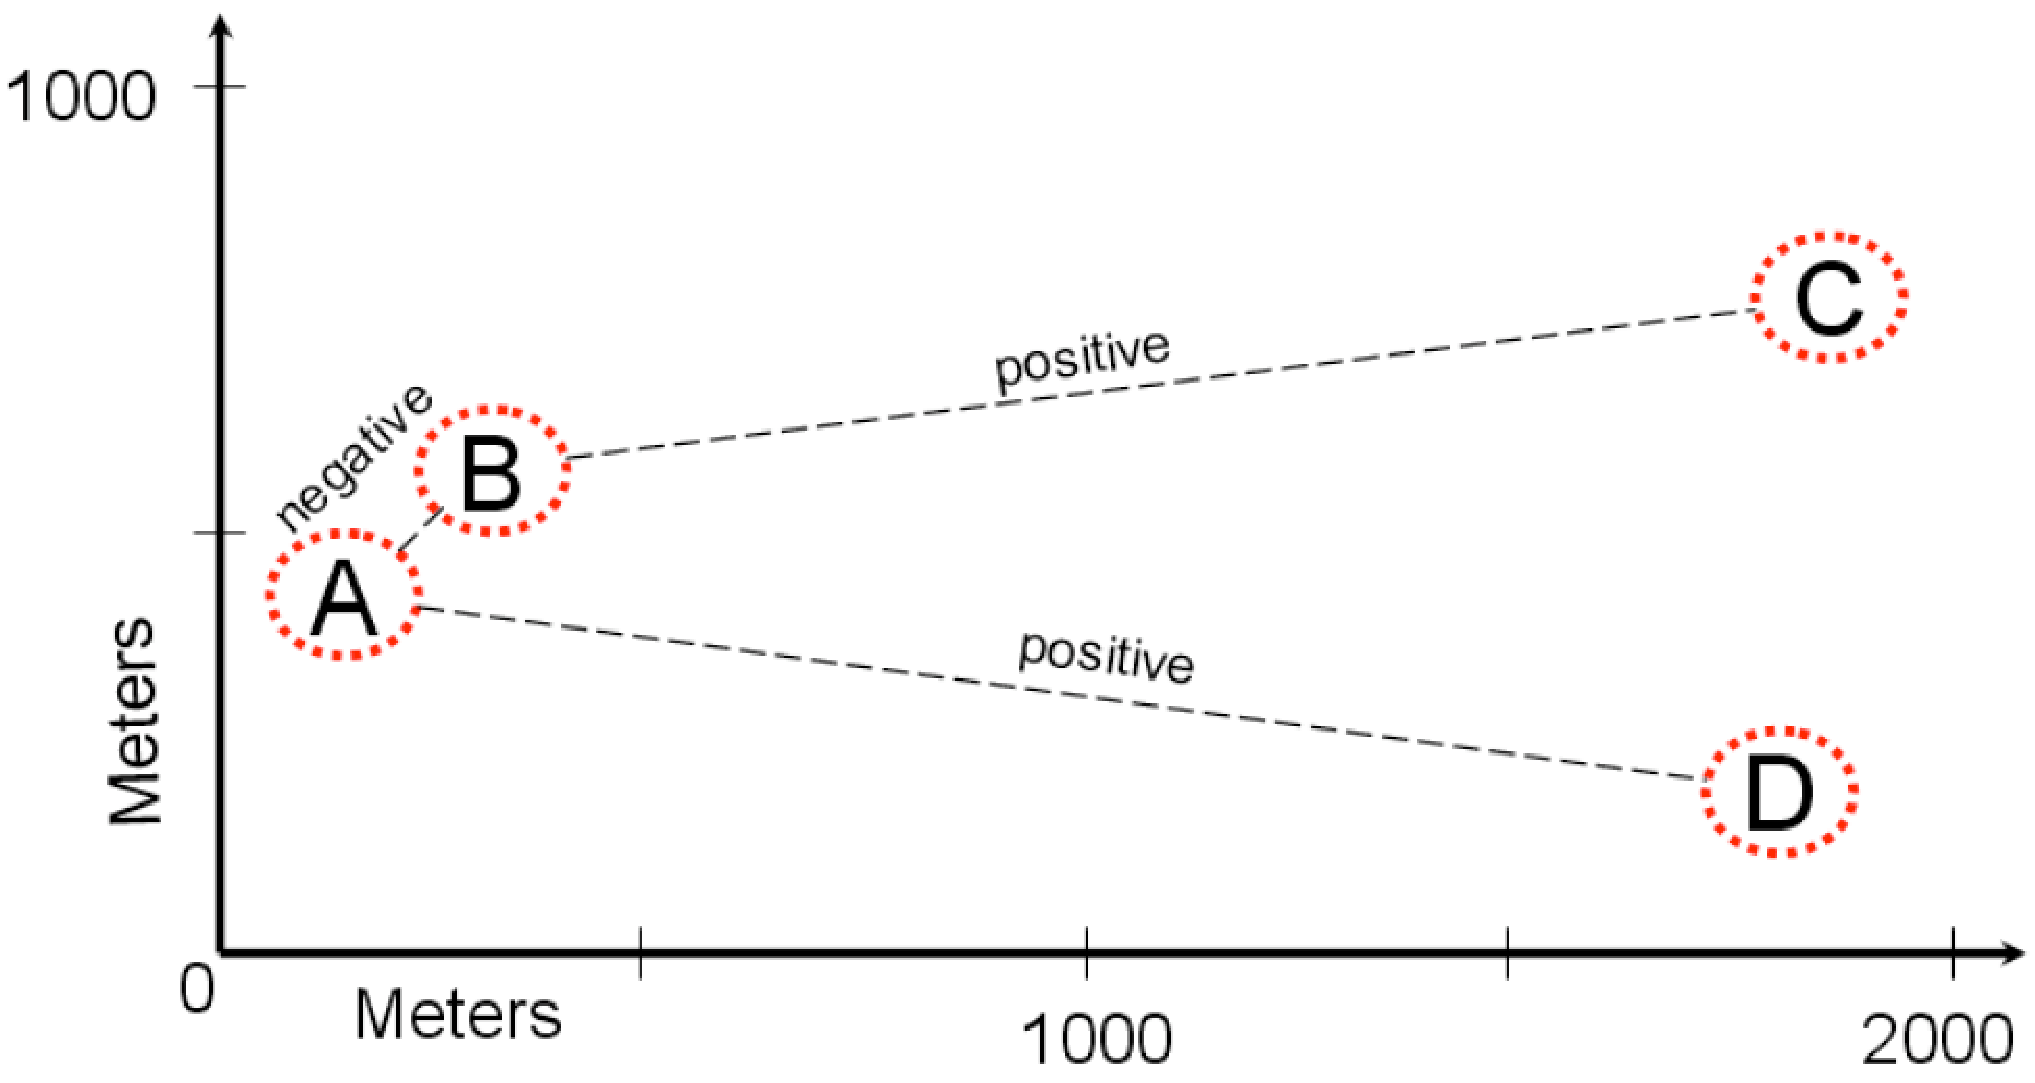
\includegraphics[width=0.7\textwidth]{../images/positive.pdf}
\end{center}
\end{frame}

\begin{frame}
\frametitle{Gang Formation}
\begin{center}
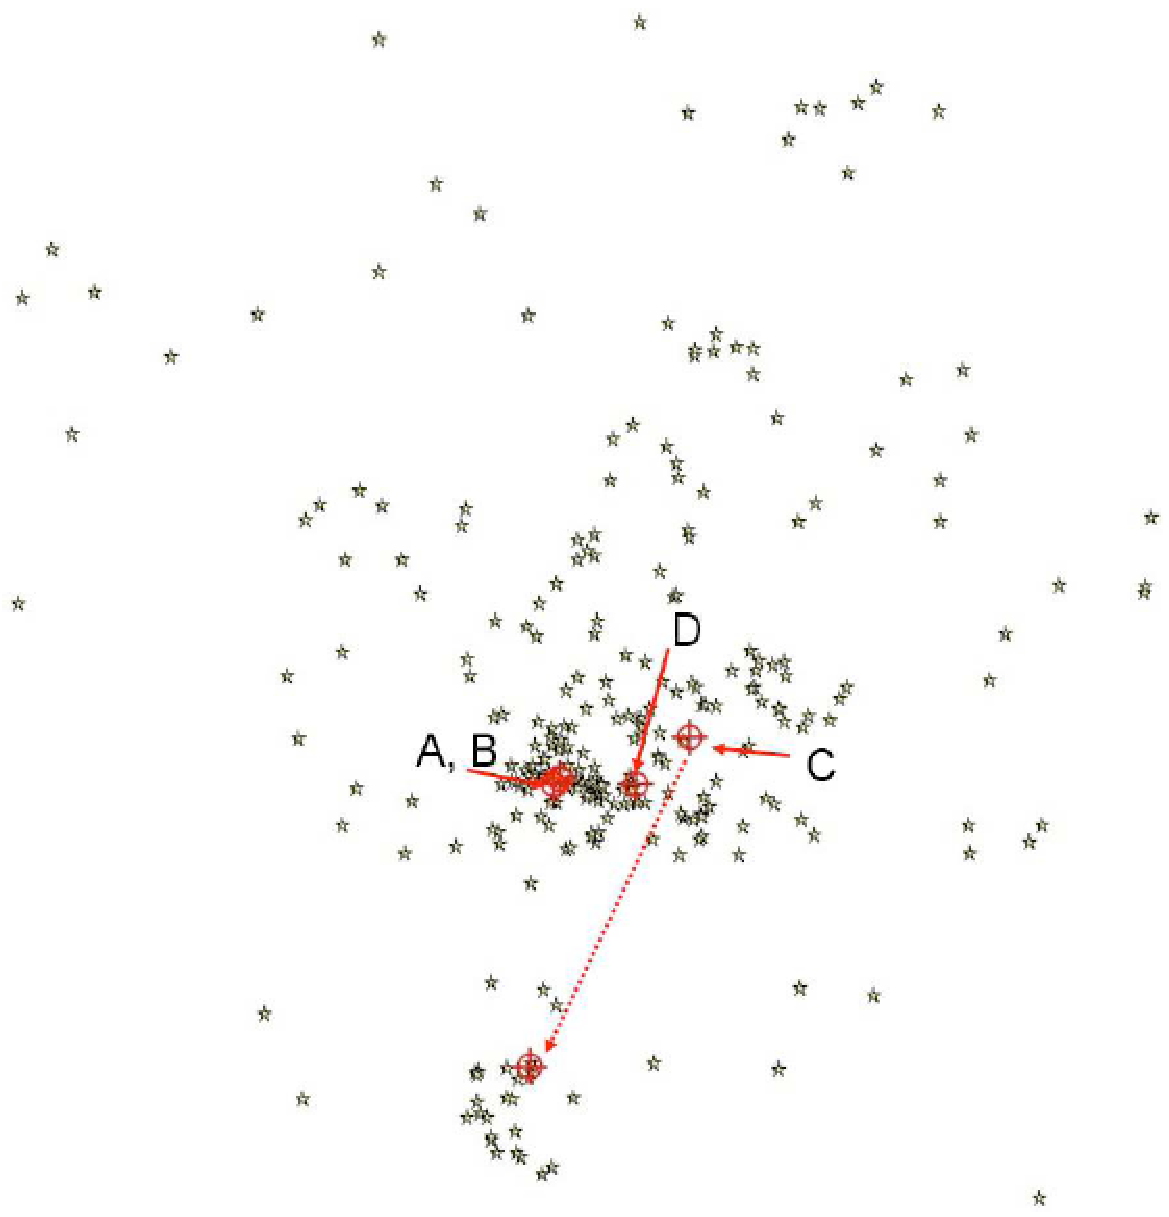
\includegraphics[width=0.5\textwidth]{../images/serious.pdf}
\end{center}
\end{frame}

\begin{frame}
\frametitle{Gangs in South Manchester, UK}
\begin{itemize}
\item All serious crimes: {\emph{murder, attempted murder, manslaughter,
  kidnapping, serious wounding, firearms offences}}. 
\item Gang C has moved into an additional location with drug selling.
\item 38\% ({\emph{n}}=162) of all serious crimes occurring within 1
  km radius (of gang locations).
\item 63\% of all serious crimes occur within 2 km.
\item 53\% ({\emph{n}}=9) of murders are within 3 km
\item 38\% ({\emph{n}}=34) of attempted murders are within 1 km, 63\% within 2 km
\item 33\% ({\emph{n}}=17) of serious woundings are within 1 km, 48\% are within 2 km. 
\end{itemize}
\end{frame}

\section{Police Databases}

{ % all template changes are local to this group.
    \setbeamertemplate{navigation symbols}{}
    \begin{frame}[plain]
        \begin{tikzpicture}[remember picture,overlay]
            \node[at=(current page.center)] {
                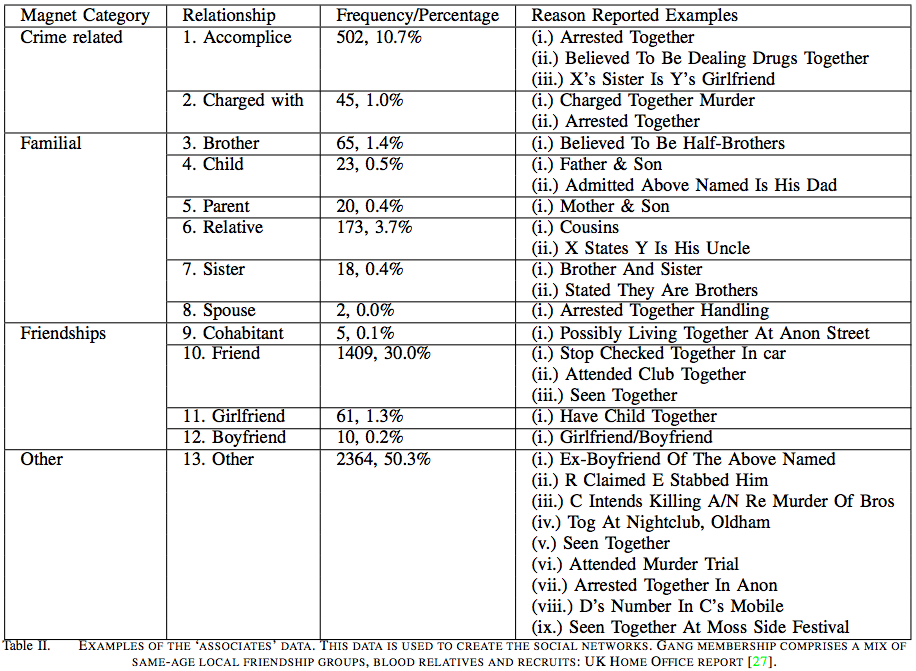
\includegraphics[width=0.9\paperwidth]{../images/associatesdata.png}
            };
        \end{tikzpicture}
     \end{frame}
}

\section{Network Characterisation}

\begin{frame}
\begin{center}
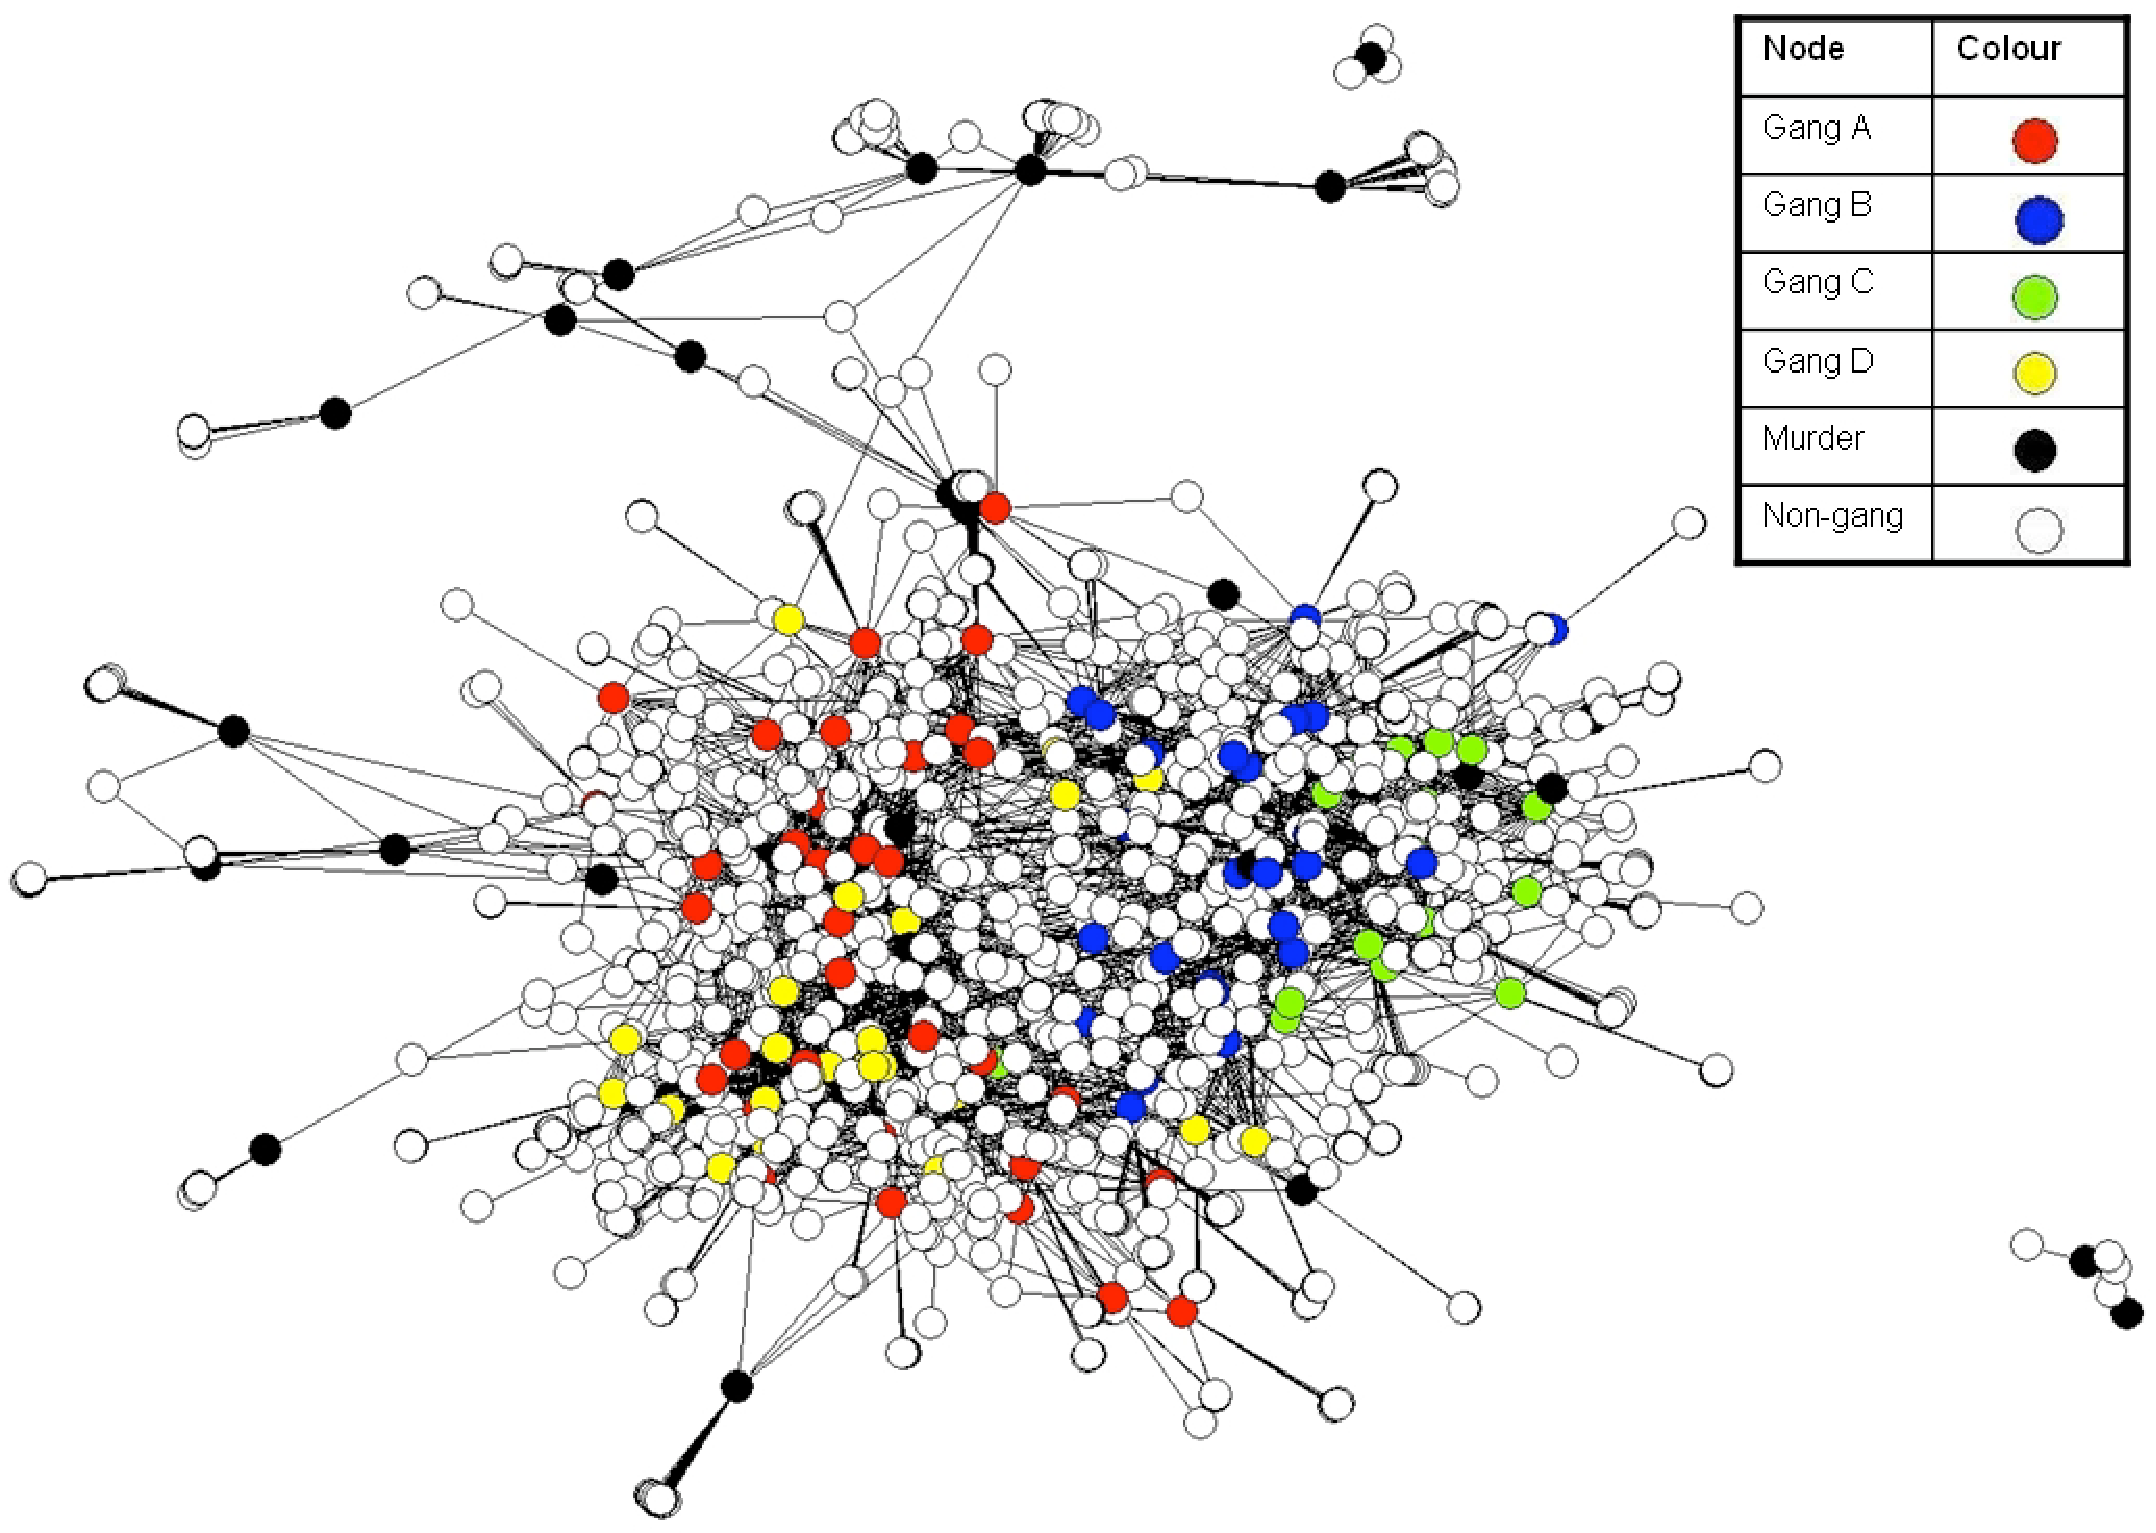
\includegraphics[width=0.7\paperwidth]{../images/legend2006.pdf}
\end{center}
\hfill\scriptsize{{\textbf{Network in 2006.}}}
\end{frame}

\begin{frame}
\begin{center}
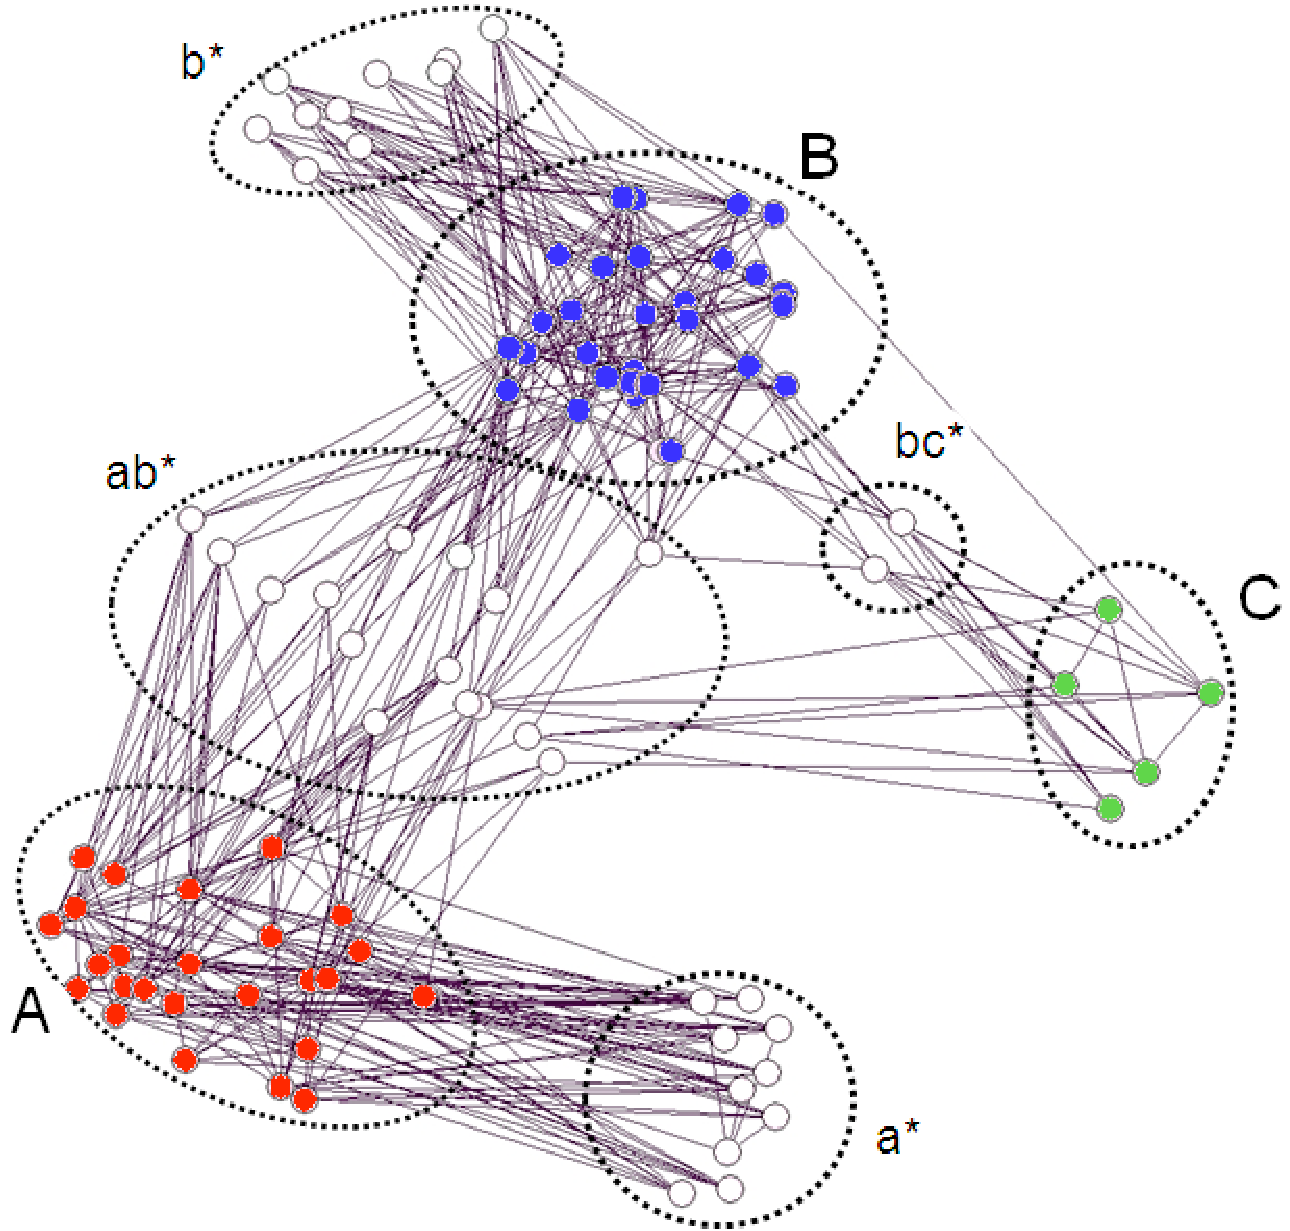
\includegraphics[width=0.6\paperwidth]{../images/2002core_labelled.pdf}
\end{center}
\scriptsize{{\textbf{Link reduction, showing Gangs A and B and emergence of Gang
C (for 2002).}} This also illustrates the large amount of non-gang members who
are associated with individual gangs ({\emph{a*, b*}}) or who are intermediaries ({\emph{ab*,
bc*}}).}
\end{frame}

\subsection{Small-World}

\begin{frame}
\frametitle{Small-World}
\begin{itemize}
\item A small-world network has both local connectivity and global reach, and is a simple connected graph {\emph{G}} exhibiting two properties:
\begin{enumerate}
\item Small characteristic path length: the presence of short-cut
  connections between some vertices results in a small characteristic
  path length {\emph{L(G)}}.
\item Large clustering coefficient: each vertex of {\emph{G}} is linked to a
  relatively well-connected set of neighbouring vertices, resulting in
  a large value for the clustering coefficient {\emph{C(G)}}.
\end{enumerate}
\pause
\item To determine whether our network is a random one or is
  small-world, we can test whether or not it has exponential
  {\emph{k}}-connectivity distribution.
\pause
\item {\textbf{We do not observe this in the data}}, however, we do see large
  clustering coefficients, and the average path lengths are always
  less than {\emph{log(n)}}. 
\item {\textbf{Based upon these two criteria we can still conclude that our
  networks have small-world characteristics.}}
\end{itemize}
\end{frame}

\subsection{Scale-Free}

\begin{frame}
\frametitle{Scale-Free}
\begin{itemize}
\item Plotting the clustering coefficient as a function of the number
  of nodes {\emph{n}}, should follow the power-law distribution for scale-free
  networks, with the clustering coefficient being roughly four times
  larger than random networks.
\item The value of the clustering coefficient for a random networks
  will be {\emph{1/n}}. 
\pause
\item We compare the values of {\emph{4/n}} against {\emph{CC}}.
\item  As the cumulative links increase from 2000 to 2006, the value
  of {\emph{CC}} generally increases (with the number of nodes {\emph{n}}) and is always
  significantly higher than the values of {\emph{4/n}}. 
\item Each of the gang values for {\emph{CC}} are also significantly higher
  than would be expected in a random network.
\end{itemize}
\end{frame}

\begin{frame}
\frametitle{Scale-Free cont.}
\begin{itemize}
\item The diameter of the network (longest path length) should be
  approximately {\emph{log(log(n))}} for scale-free networks.
\begin{itemize}
\item {\textbf{In both cases (for the gangs and the years) the real values are
  significantly higher than would be expected for a scale-free
  network.}}
\end{itemize}
\pause
\item The average path length should be approximately log(n) for
  scale-free networks. 
\begin{itemize}
\item {\textbf{For both the gangs and years data it was actually smaller
  than {\emph{log(n)}}, indicating scale-free networks.}}
\end{itemize}
\pause
\item The statistics on degree centrality were low, indicating that
  there is no group leader. 
\item As we know when Gangs C (2001) and D (2004) are formed, it is
  interesting to note that the characteristic of the networks at this
  time are that the betweeness centralisation reaches 0.2.
\item It is necessary to compare the closeness and betweenness
  averages for each gang against the value for the overall network.
\end{itemize}
\end{frame}

\subsection{Power Law Investigation}

\begin{frame}
\frametitle{Power Law Investigation}
\begin{center}
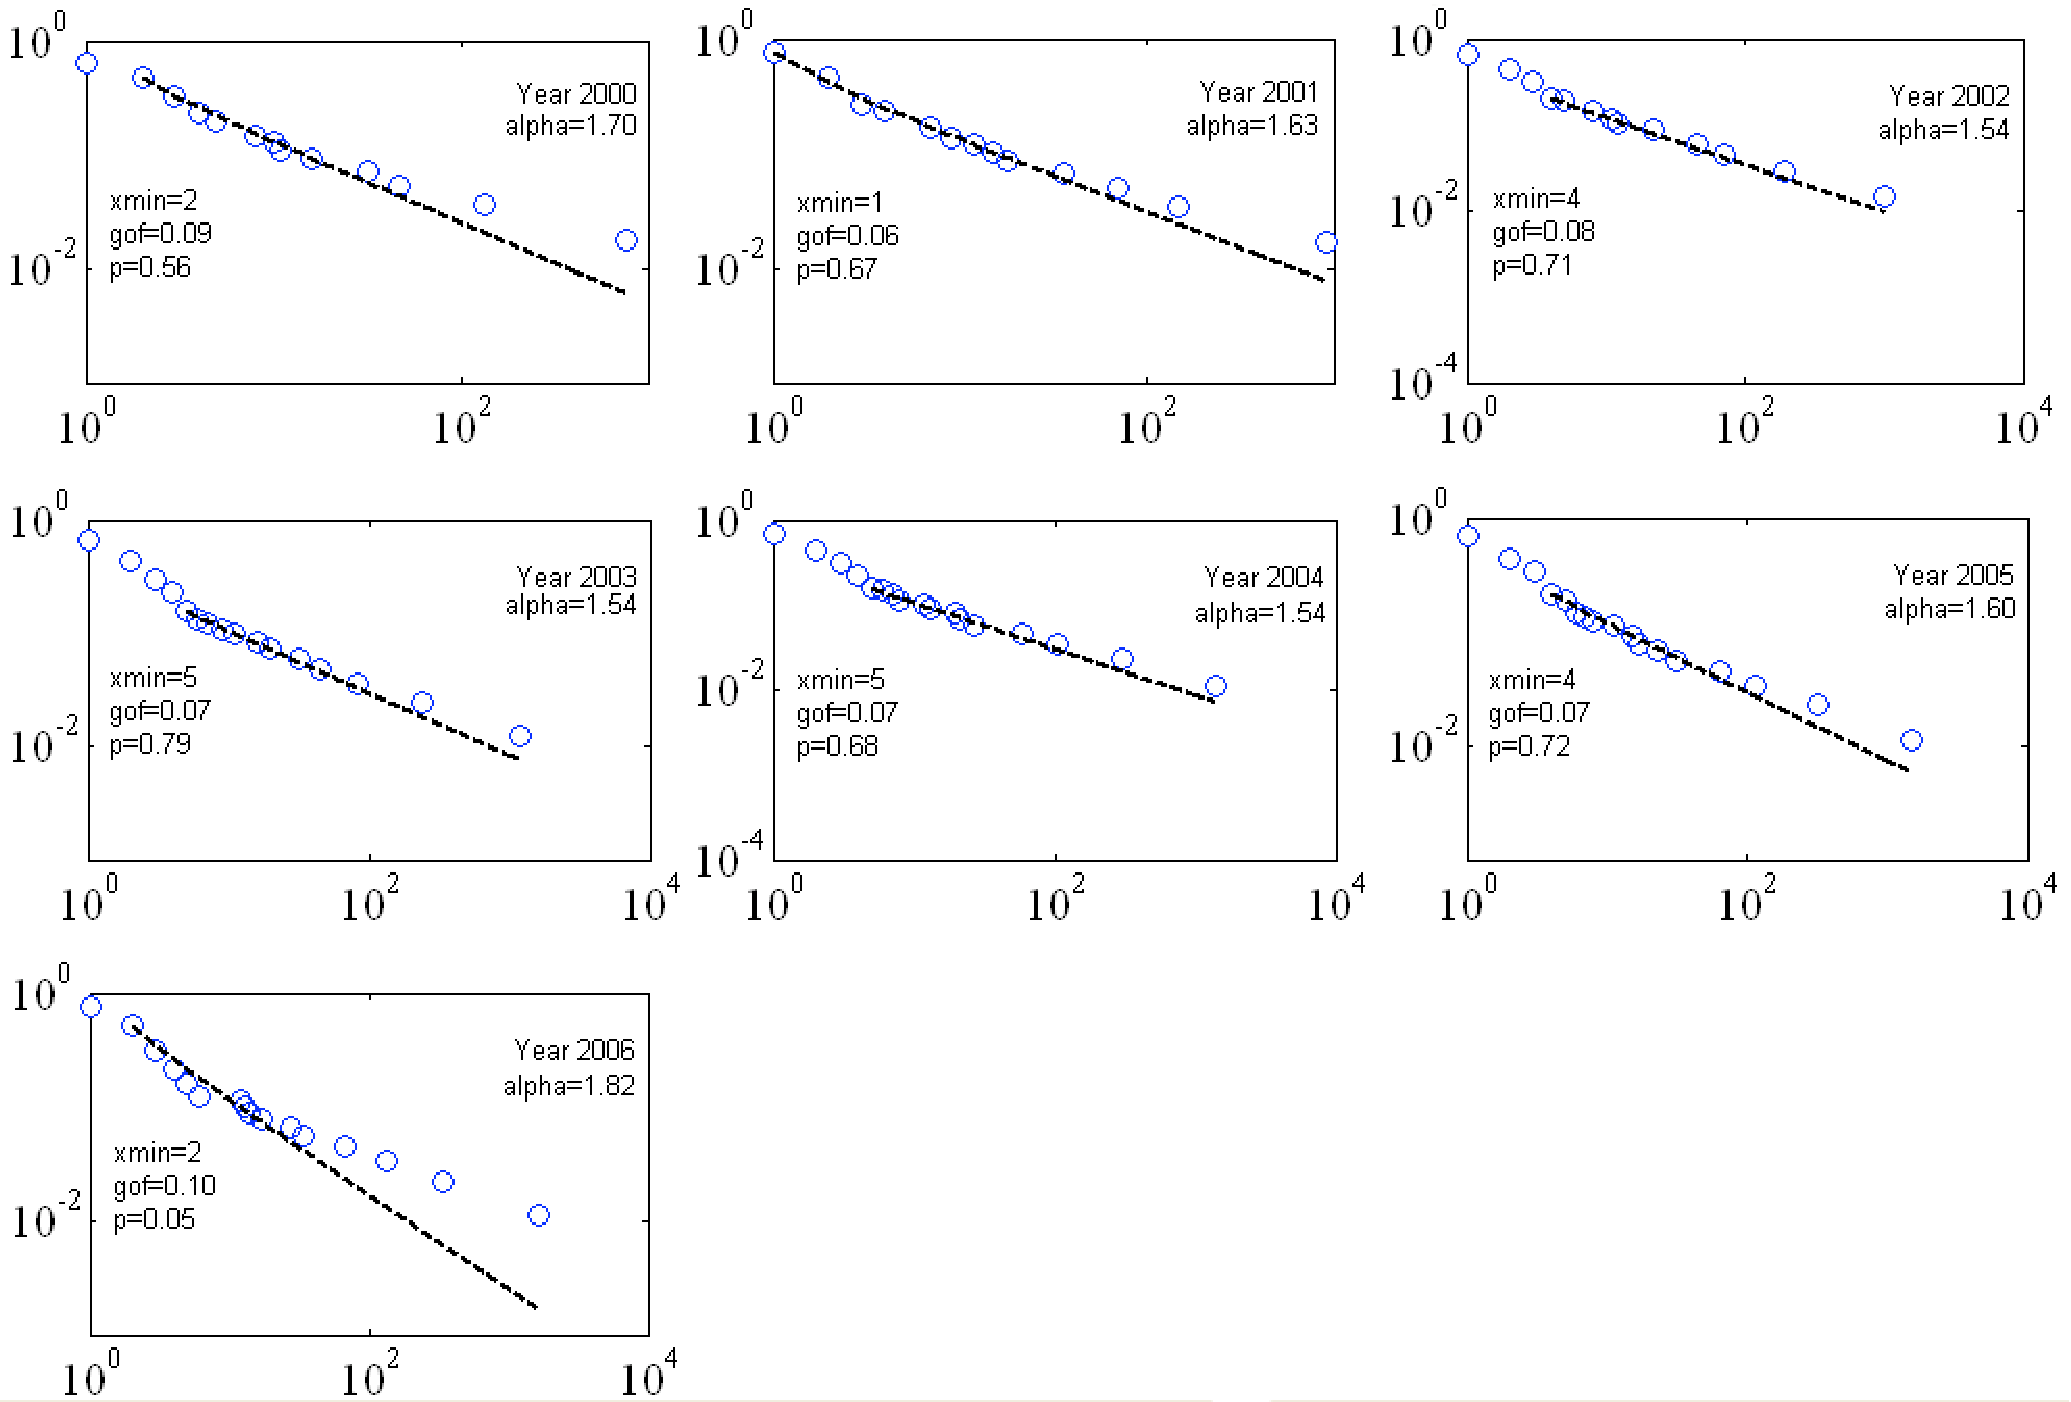
\includegraphics[width=0.9\paperwidth]{../images/clausetcumulative.pdf}
\end{center}
\end{frame}

\subsection{Emergence of Gangs}

\begin{frame}
\begin{center}
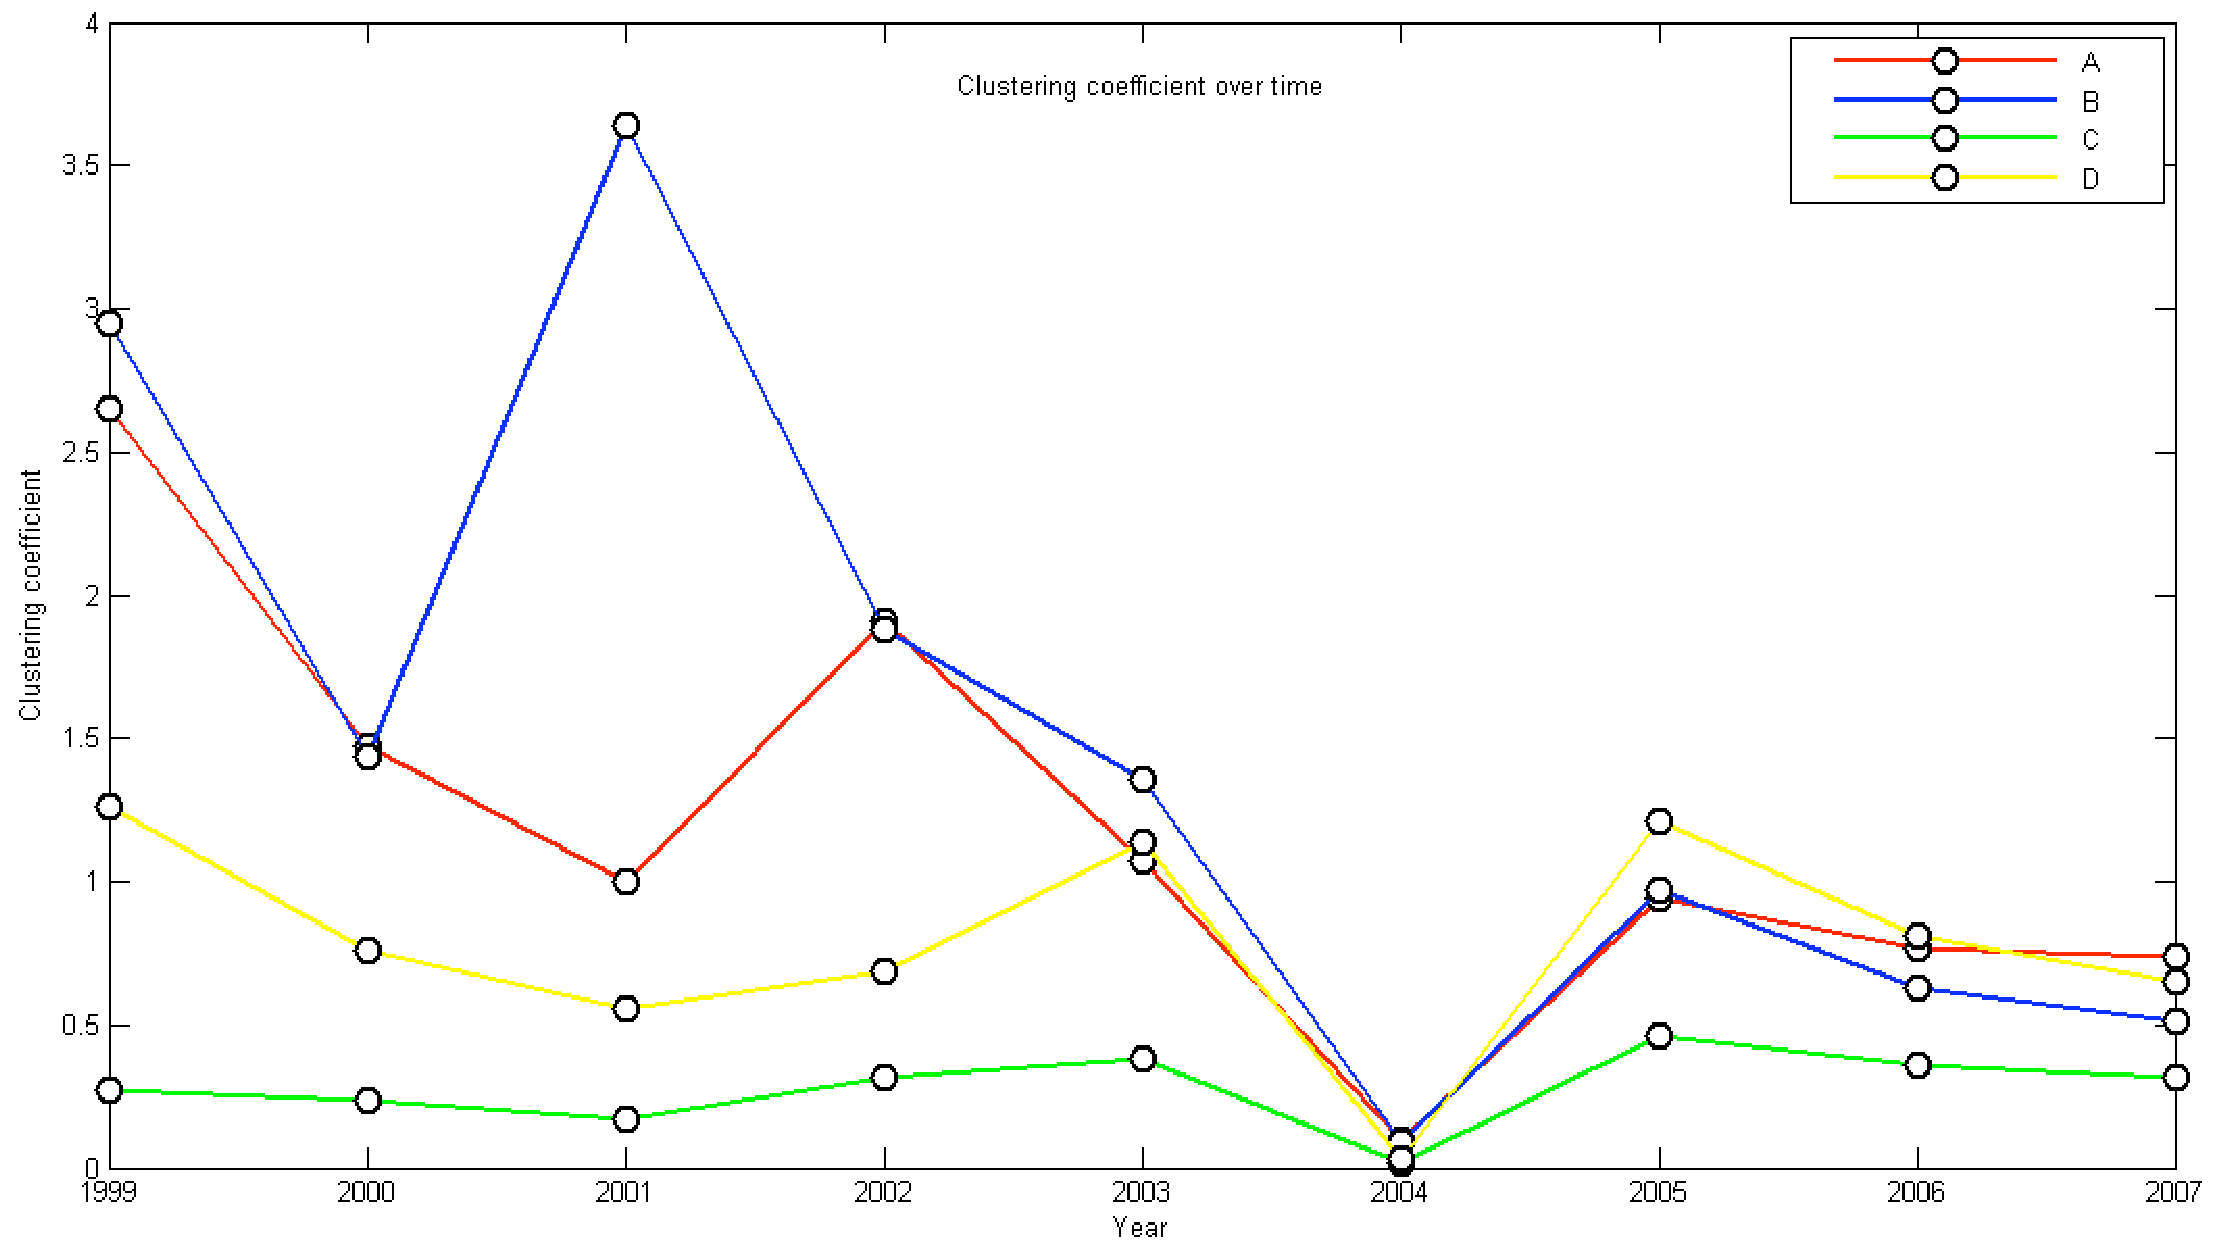
\includegraphics[width=0.9\paperwidth]{../images/gangscc1years.pdf}
\end{center}
\scriptsize{{\textbf{Per year clustering coefficients for each gang.}} Gang C was formed
in 2001, Gang D in 2004.}
\end{frame}

\begin{frame}
\begin{center}
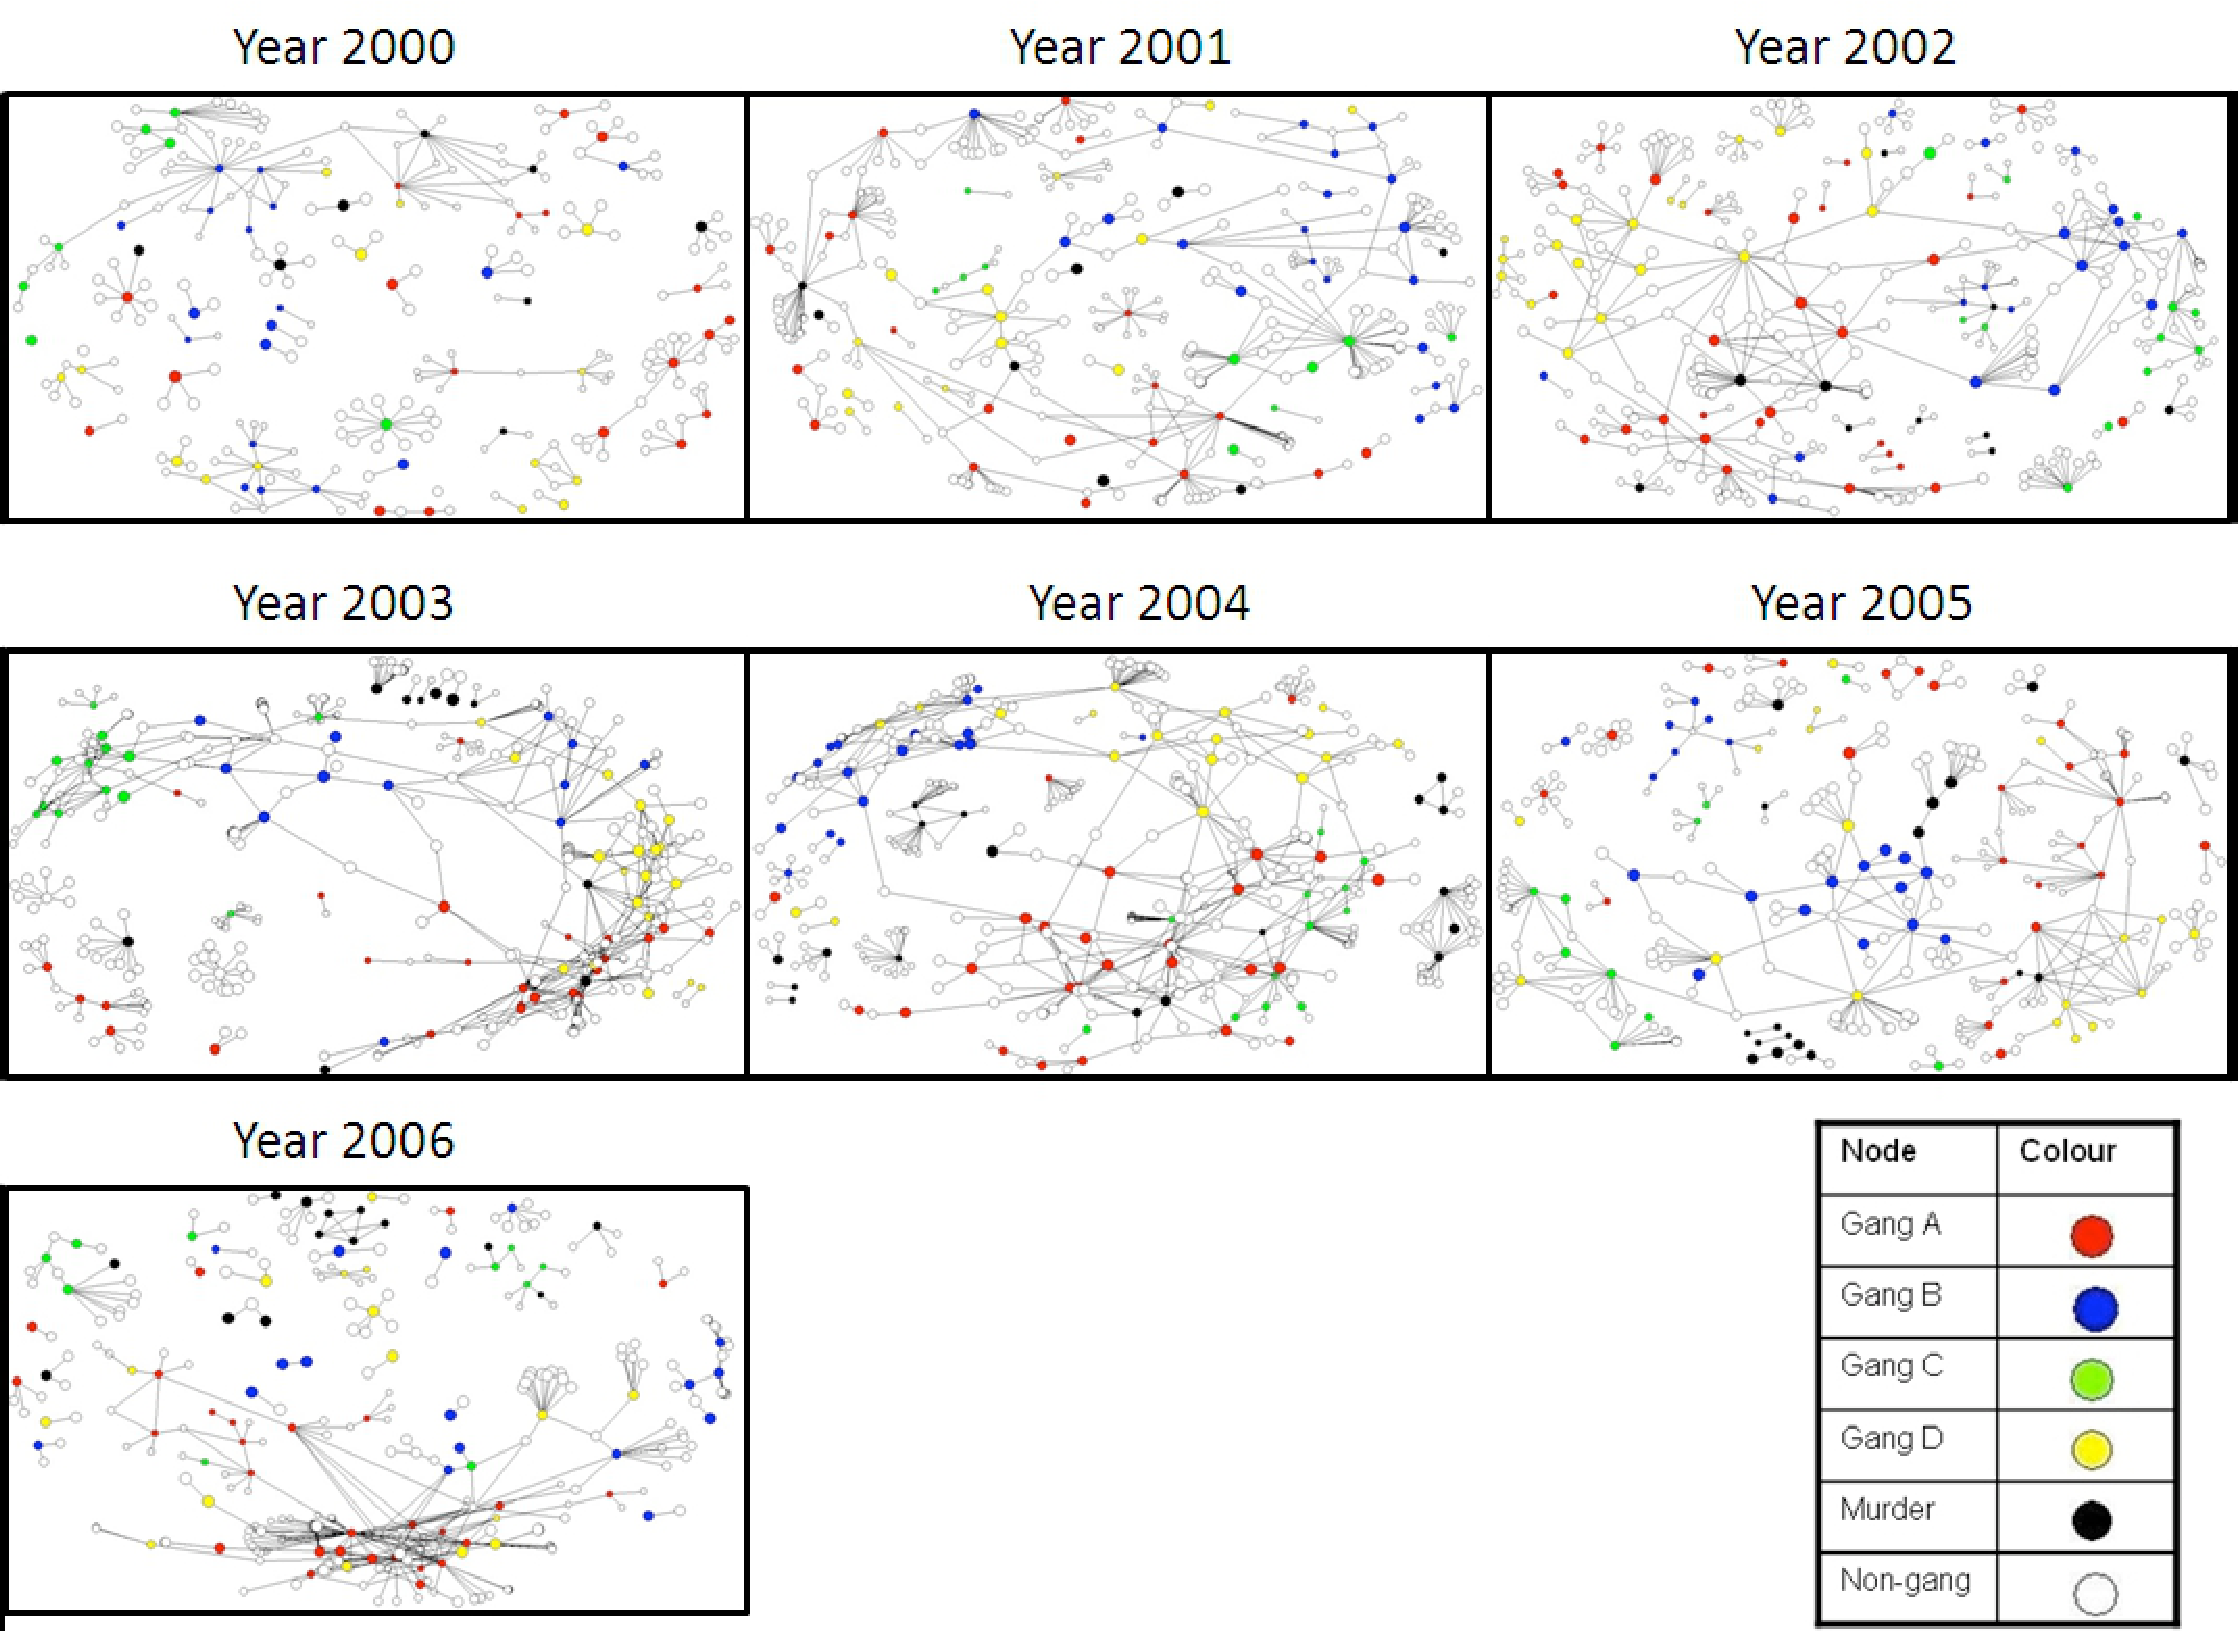
\includegraphics[width=0.8\paperwidth]{../images/all.pdf}
\end{center}
\scriptsize{{\textbf{Annual links formation.}} Only nodes directly
  connected to a gang member are included.}
\end{frame}

\section{Conclusions and Future Work}

\begin{frame}
\frametitle{Conclusions}
\begin{itemize}
\item Identifying changes can help us identify the possible birth of
  new gangs (sub-networks) in the social system.
\item Through studying the dynamics of these networks globally and
  locally, we have identified the global characteristics that tell us
  that they are not random graphs -- they are small world graphs -- 
  implying that the formation of gangs is not a random event. 
\item However, we are not yet able to conclude anything significant
  about scale-free characteristics due to insufficient sample size.
\end{itemize}
\end{frame}

\begin{frame}
\frametitle{Future Work}
\begin{itemize}
\item Further pre-processing of original data is being carried out.
\item The quality of the data collection process is to be improved.
\item Criminal behaviour (modus operandi and offence profiling) is to
be incorporated into the social network analysis.
\item {\textbf{There is significant future work available with this dataset.}}
\end{itemize}
\end{frame}

\begin{frame}
\frametitle{Acknowledgements}
\begin{itemize}
\item Acknowledge contributions from:
\begin{itemize}
\item UK EPSRC Sandpit on Gun Crime
\item Xcalibre Task Force, Greater Manchester Police, UK\newline
\end{itemize}
\item Papers and presentations:
  \url{https://github.com/tomcrick/ASONAM2014}\\
\url{https://github.com/tomcrick/FOSINT-SI2014}\newline
\item Contact: \url{http://drtomcrick.com}
\end{itemize}
\end{frame}

% \begin{frame}
% \frametitle{Crime Analysis Techniques}
% \begin{itemize}
% \item {\textbf{First Generation}}
% \begin{itemize}
% \item Anacpapa charts
% \item Maps with coloured pins\newline
% \end{itemize}
% \pause
% \item {\textbf{Second Generation}}
% \begin{itemize}
% \item Pajek
% \item IBM i2 COPLINK2, IBM i2 Analyst’s Notebook3, ORA
% \item Detica NetReveal\newline
% \end{itemize}
% \pause
% \item {\textbf{Third Generation?}}
% \end{itemize}
% \end{frame}

% \begin{frame}
% \frametitle{Crime Analysis Techniques}
% ``{\emph{Social network analysis of the sort we could call ‘third-generation’
% would focus much more intensely on the content of the contacts, on the
% social context, and on the interpretation of such information.}}''
% (Klerks, 2001)\newline\newline

% ...understanding in a qualitative way the {\textbf{behaviour, motivations and
% choices}} of the individuals concerned and contributing to a better
% understanding of vital {\textbf{social processes, power and affinity structures}}.
% \end{frame}

% \section{UK Crime Networks}

% \begin{frame}
% \frametitle{UK Crime Networks}
% {\Large{
% \begin{enumerate}
% \item Burglary\newline
% \item Gun Gangs\newline
% \item Retail Theft\newline
% \end{enumerate}}}
% \end{frame}

% \subsection{Burglary}

% \begin{frame}
% \frametitle{Burglary}
% \begin{itemize}
% \item In conjunction with {\textbf{West Midlands Police, UK}}
% \item Large network of linked offenders ({\emph{n}}=17000)
% \item The picture painted by the initial social network plot is
% somewhat misleading...
% \item While betweenness metric useful, need to consider spatial and other features (temporal/frequency) to
%   start to understand the meaning of the links between offenders
% \end{itemize}
% \end{frame}

% % { % all template changes are local to this group.
% %     \setbeamertemplate{navigation symbols}{}
% %     \begin{frame}[plain]
% %         \begin{tikzpicture}[remember picture,overlay]
% %             \node[at=(current page.center)] {
% %                 \includegraphics[width=0.9\paperwidth]{../images/burglary.pdf}
% %             };
% %         \end{tikzpicture}
% %      \end{frame}
% % }

% \begin{frame}
% %\frametitle{Geographical Networks of Burglars}
% \begin{center}
% \includegraphics[width=0.7\paperwidth]{../images/burglary.pdf}
% \end{center}
% \scriptsize{{\textbf{Geographical networks of burglars.}} Each of the 2x2 squares represents an offender, with
%   Unique Reference Number (URN), number of crimes (N) and betweeness
%   value (B). The links between offenders are labelled with dates, as days from the start of the project.}
% \end{frame}

% \subsection{Gun Gangs}

% { % all template changes are local to this group.
%     \setbeamertemplate{navigation symbols}{}
%     \begin{frame}[plain]
%         \begin{tikzpicture}[remember picture,overlay]
%             \node[at=(current page.center)] {
%                 \includegraphics[width=\paperwidth]{../images/bbcnewsmanc2004.png}
%             };
%         \end{tikzpicture}
%      \end{frame}
% }

% \begin{frame}
% \frametitle{Gun Gangs}
% \begin{itemize}
% \item In conjunction with {\textbf{Greater Manchester Police, UK}}
% \item Area with a significant gun crime problem, related to gang activity
% \item Dynamics of four gangs and their associates
% \item Value of SNA for gang research:
% \begin{itemize}
% \item Identifying structural holes
% \item Betweenness
% \item Social capital
% \end{itemize}
% \item Value of third generation analysis
% \end{itemize}
% \end{frame}

% % { % all template changes are local to this group.
% %     \setbeamertemplate{navigation symbols}{}
% %     \begin{frame}[plain]
% %         \begin{tikzpicture}[remember picture,overlay]
% %             \node[at=(current page.center)] {
% %                 \includegraphics[width=0.9\paperwidth]{../images/2000ganglabels.pdf}
% %             };
% %         \end{tikzpicture}
% %      \end{frame}
% % }

% \begin{frame}
% \begin{center}
% \includegraphics[width=0.8\paperwidth]{../images/2000ganglabels.pdf}
% \end{center}
% \scriptsize{{\textbf{Links between two rival gangs A and B.}} In 2000,
%   Gangs A and B were rivals. These later divided in 2001 into Gang C
%   (from A) and into Gang D (from B) in 2004.}
% \end{frame}

% { % all template changes are local to this group.
%     \setbeamertemplate{navigation symbols}{}
%     \begin{frame}[plain]
%         \begin{tikzpicture}[remember picture,overlay]
%             \node[at=(current page.center)] {
%                 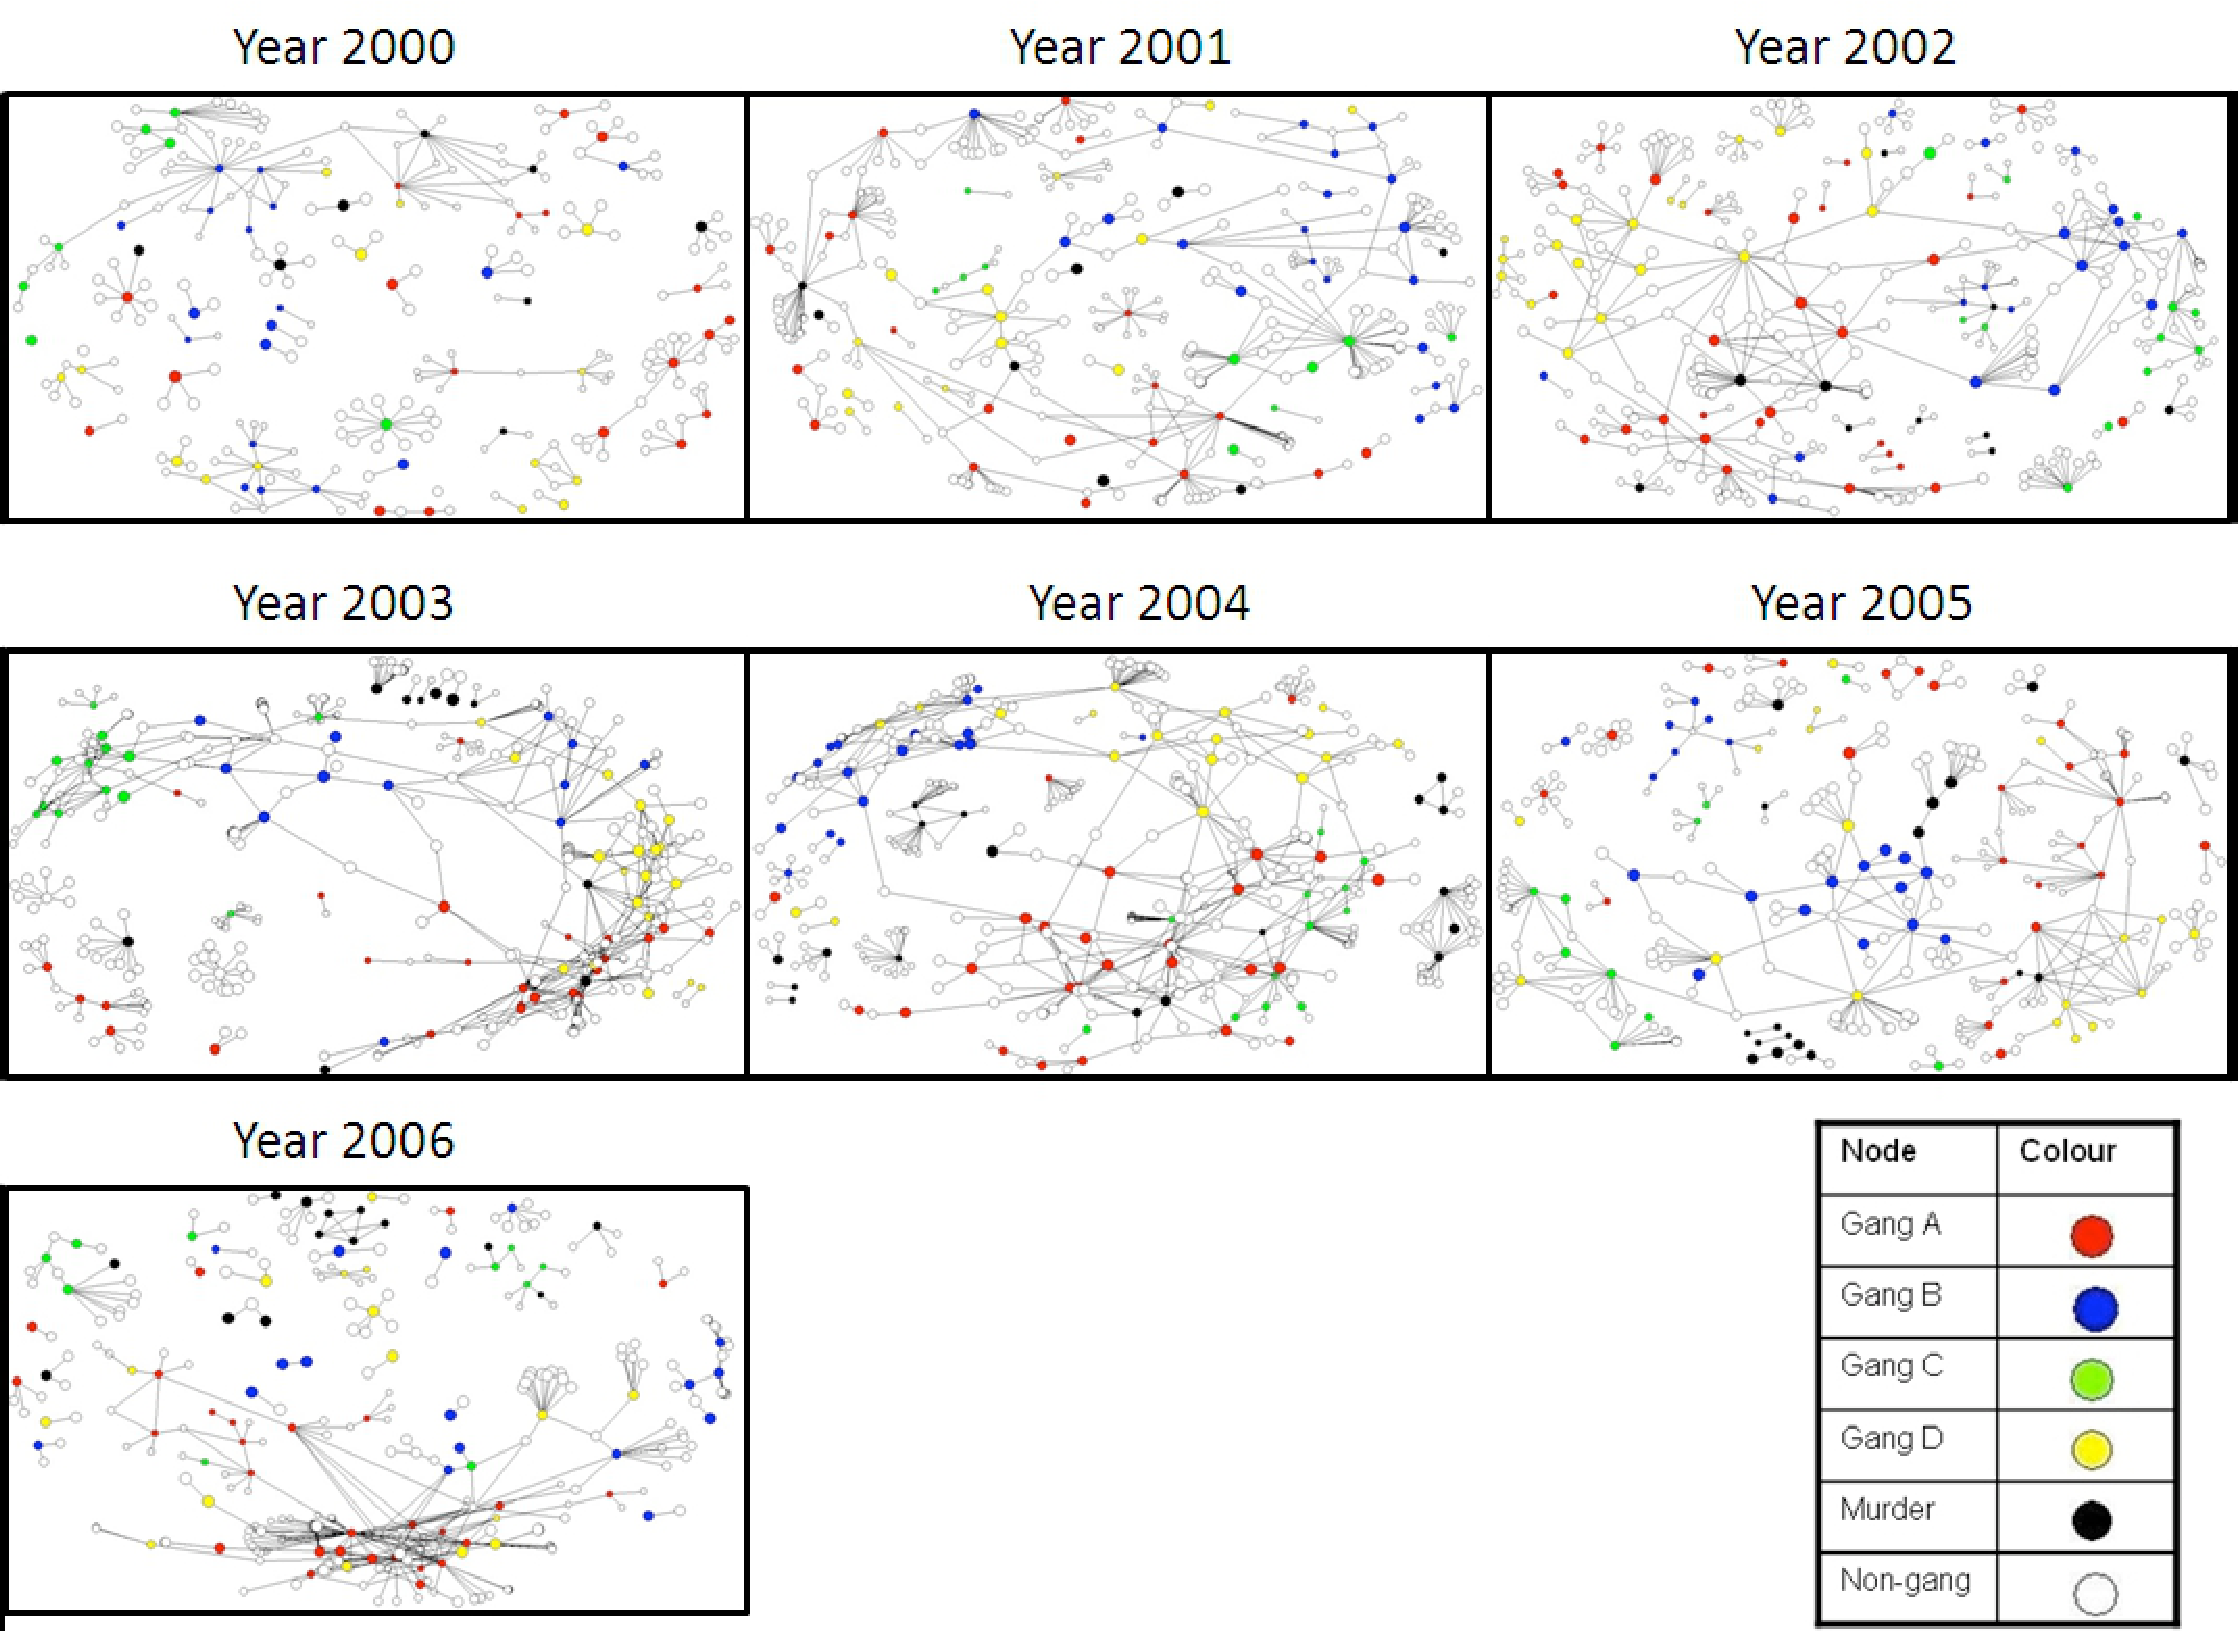
\includegraphics[width=0.9\paperwidth]{../images/all.pdf}
%             };
%         \end{tikzpicture}
%      \end{frame}
% }

% \begin{frame}
% \frametitle{Specific Gang Roles}
% \begin{itemize}
% \item {\textbf{Leader:}}
% \begin{itemize}
% \item responsible for recruiting new members
% \end{itemize}
% \item {\textbf{Provider:}}
% \begin{itemize}
% \item an individual either internal or external to the gang able to
%   supply firearms and/or ammunition
% \end{itemize}
% \item {\textbf{Enforcers/Riders:}}
% \begin{itemize}
% \item nominated individuals who are active gunmen for the gang
% \end{itemize}
% \item {\textbf{Runners/Dealers:}}
% \begin{itemize}
% \item members of the gang who distribute/supply drugs, usually on the
%   leader's behalf; younger members of the group
% \end{itemize}
% \end{itemize}
% \end{frame}

% \begin{frame}
% \frametitle{Link Analysis}
% \begin{center}
% 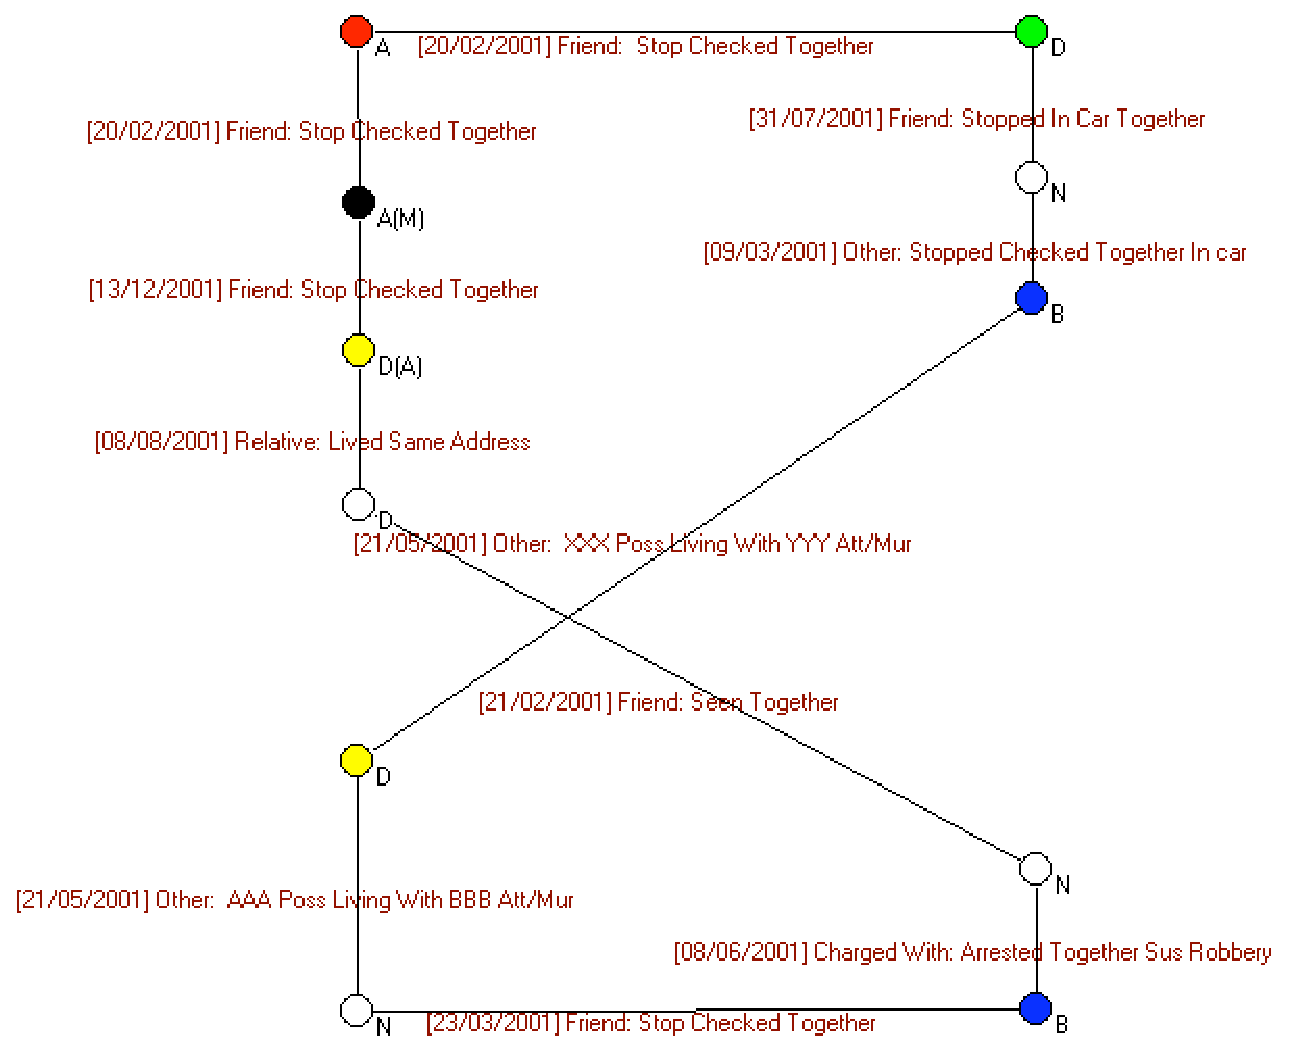
\includegraphics[width=0.48\textwidth]{../images/chain2001.pdf}
% \hfill
% 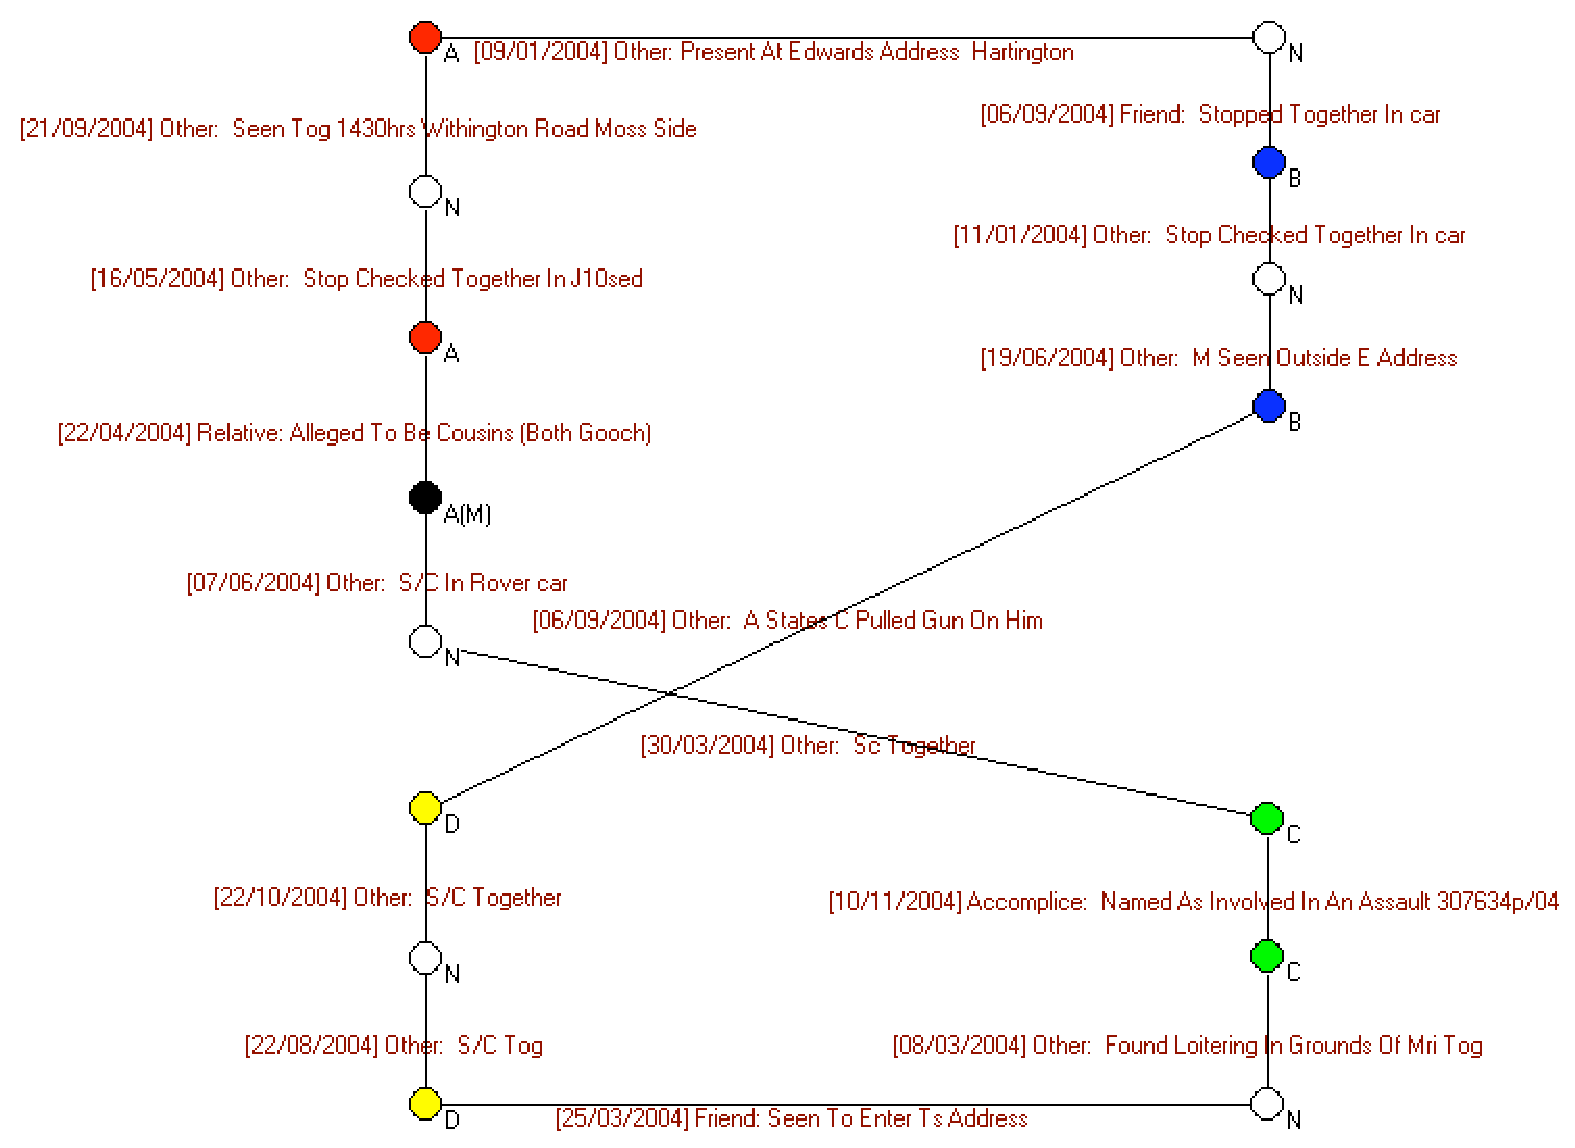
\includegraphics[width=0.48\textwidth]{../images/chain2004.pdf}
% \end{center}
% \scriptsize{{\textbf{Cycle (2001).}} The tension is between Gangs A
% (red), B (blue), C (green) and D (yellow). A(M) is a member of the
% Gooch gang (Gang A), however they are coloured black to represent the
% crime of murder.}
% \end{frame}

% { % all template changes are local to this group.
%     \setbeamertemplate{navigation symbols}{}
%     \begin{frame}[plain]
%         \begin{tikzpicture}[remember picture,overlay]
%             \node[at=(current page.center)] {
%                 \includegraphics[width=0.9\paperwidth]{../images/offenderhistories.png}
%             };
%         \end{tikzpicture}
%      \end{frame}
% }

% \begin{frame}
% \frametitle{Gun Gangs}
% \begin{itemize}
% \item The picture painted by the initial social network plot is
% somewhat misleading...
% \item In the gun gangs, the police-held hypothesis of two rival sets
%   of gangs is potentially a misrepresentation of the much more complex
%   sets of smaller cliques and fluid changes within the larger gang
%   structures.
% \item {\textbf{Extremely rich dataset}}; more processing and analysis to follow
% \end{itemize}
% \end{frame}

% \subsection{Retail Theft}

% \begin{frame}
% \frametitle{Retail Theft}
% \begin{itemize}
% \item Unique database from the {\textbf{UK's North East Retail Crime Partnership (NERCP)}}
% \item Partnership between:
% \begin{itemize}
% \item 29 retail chains
% \item 11 shopping centres
% \item 6 town/city centre partnerships
% \item 4 police forces in the NE of England (+ 11 further forces)
% \end{itemize}
% \item Information on over 30,000 offenders and 102,000 incidents in
%   any 12 month period
% \item Complex data of retail crime, with a fraction of known
%   gangs, presents its own particular challenges -- how to make use of
%   detailed intelligence on individuals (in textual format) and
%   combine with mining of the social networks.
% \end{itemize}
% \end{frame}

% % { % all template changes are local to this group.
% %     \setbeamertemplate{navigation symbols}{}
% %     \begin{frame}[plain]
% %         \begin{tikzpicture}[remember picture,overlay]
% %             \node[at=(current page.center)] {
% %                 \includegraphics[width=0.9\paperwidth]{../images/path1.pdf}
% %             };
% %         \end{tikzpicture}
% %      \end{frame}
% % }

% % { % all template changes are local to this group.
% %     \setbeamertemplate{navigation symbols}{}
% %     \begin{frame}[plain]
% %         \begin{tikzpicture}[remember picture,overlay]
% %             \node[at=(current page.center)] {
% %                 \includegraphics[width=0.9\paperwidth]{../images/path2.pdf}
% %             };
% %         \end{tikzpicture}
% %      \end{frame}
% % }

% % { % all template changes are local to this group.
% %     \setbeamertemplate{navigation symbols}{}
% %     \begin{frame}[plain]
% %         \begin{tikzpicture}[remember picture,overlay]
% %             \node[at=(current page.center)] {
% %                 \includegraphics[width=0.9\paperwidth]{../images/path3.pdf}
% %             };
% %         \end{tikzpicture}
% %      \end{frame}
% % }

% \begin{frame}
% \begin{center}
% \includegraphics[width=0.9\paperwidth]{../images/path3.pdf}
% \end{center}
% \scriptsize{{\textbf{Shortest path between Offender 51196 (Gang SEA)
%       and Offender 49467 (Gang CM).}}}
% \end{frame}


% \begin{frame}
% \frametitle{Conclusions and Future Work}
% \begin{itemize}
% \item The picture painted by the initial social network plot is somewhat
%   misleading in all three cases we have presented:
% \begin{itemize}
% \item {\textbf{Burglary:}} requires spatial data
% \item {\textbf{Gun Gangs:}} pre-existing police understanding of the gangs, not
%   complex enough
% \item {\textbf{Retail Theft:}} complex, fraction of known gangs, individual intelligence
% \end{itemize}
% \pause
% \item How to represent the changing nature of an individual is
%   something we have looked at elsewhere, and will continue to do so
% \pause
% \item Potential for shaping and influence policy in this area in
%   the UK
% \pause
% \item Also see: {\emph{Measuring UK Crime Gangs}} (ASONAM 2014, S9)
% \end{itemize}
% \end{frame}

\end{document}
